\section{Introduction}

Chapter~\ref{ch:nmrf} introduced Neural Markov Random Field (NMRF) as a structured neural inference framework for stereo matching.
By adaptively generating disparity hypotheses and refining them through neural message passing, NMRF enables efficient correspondence reasoning that resolves matching ambiguities while preserving sharp geometric discontinuities.
However, accurate depth learning depends not only on the model architecture, but also on the quality of ground-truth label.
In real-world robotic datasets, depth annotations are often sparse, noisy, and imperfectly aligned with the reference image.
These imperfections can significantly affect the geometry learned by stereo networks.

Outdoor stereo datasets commonly obtain depth annotations by projecting LiDAR measurements into the camera frame.
Although these measurements provide metric depth at sampled locations, the resulting labels are sparse in the image plane and usually suffer from sensor noise, calibration error, and temporal aggregation artifacts.
These issues are especially obvious near object boundaries, where projected labels can become spatially misaligned with the RGB image.
As a result, foreground objects may appear artificially thickened ($2^\mathrm{nd}$ row in Figure~\ref{fig:pseudo-labels}), thin structures may be removed, and small holes or fine details may be filled incorrectly.
When used directly as training targets, such labels can cause the network to reproduce the same artifacts, leading to blurred depth boundaries and degraded local 3D geometry.

This chapter addresses this supervision problem through structure-aware depth completion.
The goal is to convert sparse and noisy real-world depth annotations into denser and more reliable geometry supervision.
Rather than treating the available labels as fully accurate, we regard them as partial metric measurements that should be completed and corrected with the help of dense stereo prediction and image structure.
Specifically, an adapted NMRF model provides dense disparity estimates, confidence scores, and adaptive regularization weights, while the sparse labels provide metric anchors where measurements are available.
These sources are integrated by an optimization model that encourages local geometric coherence while preserving discontinuities aligned with image structures.
The completed labels are then used as additional supervision for training the stereo network.
This strategy is particularly useful near depth discontinuities and thin structures, where sparse LiDAR annotations are most likely to be unreliable.
Compared with direct training on sparse labels, structure-aware completion provides supervision that is denser, better aligned with visual boundaries, and less affected by annotation noise.
As a result, the trained model produces disparity maps with sharper boundaries and improved local surface quality.

The main contribution of this chapter are summarized as follows.
First, we analyze the effect of sparse and noisy real-world depth annotations on stereo learning, with particular attention to boundary thickening and degraded local geometry.
Second, we introduce a structure-aware depth completion formulation that combines sparse depth labels, dense NMRF predictions, confidence estimation, and image-guided geometric regularization.
Third, we show that the completed labels provide robust geometry supervision, improving disparity accuracy, boundary quality, and surface normal estimation under imperfect real-world annotations.

\section{From Sparse Labels to Robust Geometry Supervision}
Large-scale depth labels are essential for training modern stereo networks.
Synthetic datasets provide dense and accurate disparity labels, but their appearance statistics often differ from real-world scenes.
Real-world datasets better reflect deployment conditions, but their annotations are usually sparse and imperfect.
This creates a central tension in depth estimation: synthetic labels are geometrically accurate but visually less realistic, while real-world labels are visually relevant but often incomplete and noisy.
In autonomous driving datasets, depth labels are commonly obtained by projecting multi-frame aggregated LiDAR points into the camera frame.
Because LiDAR and cameras have different viewpoints and sampling pattern, the projected labels do not always align perfectly with image structures.
Moreover, many datasets increase label density by accumulating LiDAR scans across multiple frames.
Although this procedure provides more measurements, it also introduces errors when pose estimation, calibration, or dynamic-object handling is imperfect.
These errors often manifest as expanded object boundaries or misplaced depth discontinuities.
Such artifacts are harmful because depth prediction networks are trained imitate the provided supervision.
If a foreground object boundary is thickened in the label, the network may learn to predict a similarly expanded disparity pattern.
This produces bleeding artifacts in reconstructed point clouds and propagates errors to downstream 3D perception.
Therefore, robust depth learning requires not only a strong neural network, but also ground-truth depth labels that accurately captures the underlying scene geometry.
A natural remedy is to complete and refine sparse labels before using them for training.
However, depth completion is itself challenging.
Sparse measurements alone cannot determine dense geometry, while dense predictions from a pretrained network may fail under domain shift, occlusion, reflection, or weak texture.
The proposed approach resolves this ambiguity by combining both source within a structure-aware optimization framework.
Sparse labels provide metric constraints, dense NMRF predictions provide plausible geometry, and image-guided regularization encourages the completed depth to adhere to scene structure.

\section{Structure-Aware Depth Completion}
Given a rectified stereo image pair, let $d\in\mathbb{R}^{\Omega}_+$ denote the dense disparity predicted by a pretrained NMRF model over the image domain $\Omega$.
The model also predicts a confidence map $w\in[0,1]^{\Omega}$, where larger values indicate more reliable predictions.
In addition, an adaptive regularization weight $\alpha_1\in\mathbb{R}^{\Omega}_{+}$ is estimated to modulate the strength of local smoothness.
Let $d^{\mathrm{gt}}$ denote the sparse ground-truth disparity labels provided by the dataset.
Our goal is to estimate a completed disparity map $u\in\mathbb{R}^{\Omega}_+$ that satisfies three requirements.
It should preserve the metric information from available ground-truth sparse labels, remain close to reliable dense NMRF predictions, and maintain local geometric coherence without oversmoothing true depth discontinuities.
We formulate this objective as
\begin{equation}
	\min_{u}
	\;
	R(u; I^L)
	+
	G(u; d, w),
	\label{eq:sadc-energy}
\end{equation}
where $G(u;d,w)$ is a confidence-weighted data term and $R(u;I^L)$ is an image-aware geometric regularizer.

The dense NMRF prediction provides useful geometry in regions where sparse labels are unavailable.
However, these predictions should not be trusted uniformly.
We therefore weight their influence using the predicted confidence map:
\begin{equation}
	G(u; d, w)
	=
	\int_{\Omega}
	\frac{1}{2} w(x)
	\bigl(u(x)-d(x)\bigr)^2
	\mathrm{d}x .
	\label{eq:sadc-data}
\end{equation}
When $w(x)$ is high, the completed disparity is encouraged to follow the network prediction.
When $w(x)$ is low, the optimization relies more on sparse measurements and regularization.
During pseudo-label generation, available sparse labels are used as metric anchors so that the completed disparity remains consistent with real sensor measurements.

The regularization term is designed to encourage locally coherent geometry while preserving sharp boundaries.
We adopt a second-order Total Generalized Variation (TGV)~\cite{bredies2010total} prior:
\begin{equation}
	\mathrm{TGV}_{\alpha}^{2}(u)
	=
	\min_{\mathbf{v}}
	\left\{
	\alpha_1
	\int_{\Omega}
	|\nabla u-v| \mathrm{d}x
	+
	\alpha_0
	\int_{\Omega}
	|\nabla v| \mathrm{d}x
	\right\},
	\label{eq:sadc-tgv}
\end{equation}
where $\mathbf{v}$ is an auxiliary vector field that approximates the disparity gradient.
Compared with first-order smoothness, TGV better preserves piecewise affine surfaces, which are common in man-made environments.
Standard TGV does not consider image structure and may smooth across object boundaries.
To make the regularization aware of image structures, we introduce an anisotropic diffusion tensor derived from the left image:
\begin{equation}
	T
	=
	\exp
	\left(
	-\beta |\nabla I^L|^{\gamma}
	\right)
	nn^{\top}
	+
	n^{\perp}{n^{\perp}}^{\top},
	\label{eq:sadc-tensor}
\end{equation}
where $n=\nabla I^L/|\nabla I^L|$ denotes the image gradient direction, $n^{\perp}$ is its orthogonal counterpart, and $\beta$, $\gamma$ are hyperparameters controling the tensor's magnitude and sharpness.
This tensor suppress smoothing along the image gradient direction $n$ while promoting smoothness in the orthogonal direction $n^{\perp}$, to better align disparity transitions with image edges.
Combining the data term and the regularizer gives the final completion objective:
\begin{equation}
	\begin{aligned}
		\min_{u,v}
		\quad
		&
		\int_{\Omega} \alpha_1(x)
		|T(\nabla u-v)| \dd x
		+
		\alpha_0
		\int_{\Omega}
		|\nabla v| \dd x
		\\
		&
		+
		\int_{\Omega}
		\frac{1}{2}w(x)
		\bigl(u(x)-d(x)\bigr)^2 \dd x .
	\end{aligned}
	\label{eq:sadc-final-energy}
\end{equation}
The spatially varying weight $\alpha_1$ allows the regularization strength to adapt to local image and disparity structures.

\section{Primal-Dual Optimization}
The proposed optimization problem Equation~\ref{eq:sadc-final-energy} is convex but non-smooth due to the TGV regularizer.
To efficiently solve it, we adopt it through the first-order primal-dual algorithm proposed by~\cite{chambolle2011first}.
By introducing dual variables $p$ and $q$, the problem can be reformulated as a convex-concave saddle point problem using the Legendre-Fenchel transform:
\begin{equation}
	\begin{aligned}
		\min_{u,v}
		\max_{p\in\mathcal{P},q\in\mathcal{Q}}
		\quad
		&
		\alpha_1
		\langle T(\nabla u-v),p\rangle
		+
		\alpha_0
		\langle \nabla v,q\rangle
		\\
		&
		+
		\sum_{(i,j)\in\Omega}
		\frac{1}{2}w_{ij}(u_{ij}-d_{ij})^{2}.
	\end{aligned}
	\label{eq:sadc-saddle}
\end{equation}
Here $p$, $q$ are dual variables with feasible sets
\begin{equation}
	\mathcal{P}
	=
	\{p:\Omega\rightarrow\mathbb{R}^{2}
	\mid
	\|p_{ij}\|\leq 1\},
	\qquad
	\mathcal{Q}
	=
	\{q:\Omega\rightarrow\mathbb{R}^{4}
	\mid
	\|q_{ij}\|\leq \alpha_0\}.
\end{equation}
This reformulation enables iterative updates of primal and dual variables for each pixel.
Optimization proceeds via gradient-ascent on $q$ and $q$, followed by gradient-descent on $u$ and $v$.
Additionally, over-relaxation is applied to the primal variables to ensure convergence.

The variables are initialized as follows: $u^0=d$, $v^0=p^0=q^0=0$.
In practice, a fixed number of iterations is sufficient for generating pseudo labels.
Choose step size $\sigma_p>0$, $\sigma_q>0$, $\tau_u>0$, and $\tau_v>0$, the iterations proceed as:
\begin{equation}
	\begin{cases}
		p^{n+1}&=\mathcal{P}_p\left\{p^n+\sigma_p\alpha_1\left(T(\nabla \bar{u}^n-\bar{v}^n)\right)\right\}\\
		q^{n+1}&=\mathcal{P}_q\left\{q^n+\sigma_q \nabla \bar{v}^n\right\}\\
		u^{n+1}&=\frac{u^n+\tau_u\left(\alpha_1\nabla^\mathsf{T} Tp^{n+1} + wd\right)}{1 + \tau_u w}\\
		v^{n+1}&=v^n+\tau_v\left( \nabla^\mathsf{T} q^{n+1} + \alpha_1Tp^{n+1}\right)\\
		\bar{u}^{n+1}&=u^{n+1}+\theta (u^{n+1}-\bar{u}^n)\\
		\bar{v}^{n+1}&=v^{n+1}+\theta (v^{n+1}-\bar{v}^n)\\
	\end{cases}
	\label{eq:pd-step}
\end{equation}
The operators $\mathcal{P}_p$ and $\mathcal{P}_q$ perform pointwise Euclidean projection onto the feasible sets $P$ and $Q$:
\begin{equation}
	\mathcal{P}_p\{\tilde{p}_{i,j}\}=\frac{\tilde{p}_{i,j}}{\max(1, ||\tilde{p}_{i,j}||)},
	\mathcal{P}_q\{\tilde{q}_{i,j}\}=\frac{\tilde{q}_{i,j}}{\max(1, \nicefrac{||\tilde{q}_{i,j}||}{\alpha_0})}.
\end{equation}
We use a fixed relaxation parameter $\theta=1$.
The gradient operator $\nabla$ and divergence operator $\nabla^\mathsf{T}$ are discretized using forward and backward differences, with Neumann and Dirichlet boundary conditions applied where appropriate.

\section{Generating Pseudo Depth Labels}

The completed disparity map should be used for training only where it is sufficiently reliable.
Although dense NMRF predictions provide useful structure, they may still be inaccurate in regions with severe domain shift, occlusion, reflections, weak texture.
Therefore, pseudo-label generation should not simply densify sparse labels everywhere.
Instead, it should selectively combine reliable dense predictions with sparse metric measurements and discard regions where the completed geometry is insufficiently supported.

\subsection{Adapting NMRF for Completion}
To provide necessary cues for structure-aware depth completion, we slightly adapt the NMRF refinement module (Section~\ref{sec:nmrf_refinement}).
In addition to predicting the refined disparity map $d$, the network is extended to estimate two auxiliary maps: a confidence map $w$ and an adaptive regularization coefficient $\alpha_1$.
These maps are not used as final depth outputs.
Rather, they guide the depth completion process by determining where the dense prediction should be trusted and how strongly local smoothness should be imposed.

The confidence map $w\in[0,1]^{\Omega}$ measures the reliability of the dense disparity prediction.
A large value indicates that the prediction is likely to provide a useful constraint in the completion objective, while a small value weakens the influence of the network prediction.
For numeric stability, the network predicts an unconstrained variable $s$ and maps it to the confidence in log-space:
\begin{equation}
	w(x)=\exp\bigl(-s(x)\bigr),
	\qquad
	s(x)\in[0,10].
\end{equation}
This parameterization ensures positive confidence values and avoid numeric instability as we directly regress aleatoric uncertainty in log space.
The adaptive coefficient $\alpha_1$ controls the strength of the first-order term in the structure-aware regularizer.
Intuitively, large $\alpha_1$ encourages stronger local geometric coherence, while small $\alpha_1$ relaxes the smoothness constraint near likely discontinuities or complex structures.
The network predicts another variable $\zeta$ and maps it into a bounded interval:
\begin{equation}
	\alpha_1(x)
	=
	\alpha_1^{-}
	+
	\bigl(\alpha_1^{+}-\alpha_1^{-}\bigr)
	\sigma\bigl(\zeta(x)\bigr),
	\label{eq:sadc-alpha}
\end{equation}
where $\sigma(\cdot)$ denotes the sigmoid function, and $\alpha_1^{-}$ and $\alpha_1^{+}$ define the minimum and maximum regularization strengths.
In practice, these maps are decoded from the fine-level NMRF features using a lightweight prediction head parallel to the disparity residual head.
This design allows the completion model to use not only the disparity prediction itself, but also the network's estimate of prediction reliability and local geometric complexity.

With this adaption, the pretrained NMRF model provides three dense inputs for label generation:
\begin{equation}
	d,\; w,\; \alpha_1
	=
	f_{\mathrm{NMRF}}(I^L,I^R),
	\label{eq:sadc-nmrf-cues}
\end{equation}
where $d$ is the dense disparity prediction, $w$ is the confidence map, and $\alpha_1$ is the adaptive regularization coefficient.
These cues are then combined with the sparse real-world label $d^{\mathrm{gt}}$ in the structure-aware completion objective introduced in Equation~\ref{eq:sadc-final-energy}.
The confidence map $w$ and adaptive regularization coefficient $\alpha_1$ should provide meaningful cues for the structure-aware completion model.
To encourage this behavior, we introduce an auxiliary supervision signal by unrolling the primal-dual optimization steps in Equation~\ref{eq:pd-step}.
The unrolled solver is differentiable, allowing gradients to propagate through the completion process and update the NMRF branches that predict $d$, $w$, and $\alpha_1$.
Let $\hat{u}$ and $\hat{v}$ denote the outputs of the unrolled completion solver for the optimization problem.
Here, $\hat{u}$ is the completed disparity map, and $\hat{v}$ is the auxiliary field associated with local disparity variation.
A direct way to transfer the effect of the completion solver to NMRF would be to enforce consistency between the solver output $\hat{u}$ and the network prediction $d$, \ie, $|\hat{u}-d|$.
However, the completed output is not always more accurate than the network prediction.
In regions with complex non-planar geometry, very thin structures, or weak image evidence, the piecewise-affine regularization assumption may be imperfect and can over-smooth local details.
To make the auxiliary supervision robust, we anchor both the network prediction and the completed output to the available ground-truth disparity:
\begin{equation}
	L^{\textsf{aux}}
	=
	\frac{1}{|\Omega|}
	\sum_{(i,j)\in\Omega}
	\left(
	|\hat{u}_{ij}-d^{\mathrm{gt}}_{ij}|
	+
	|d_{ij}-d^{\mathrm{gt}}_{ij}|
	\right).
	\label{eq:loss-aux}
\end{equation}
This objective can be interpreted as a supervised upper bound on the direct consistency loss, since
\begin{equation}
	|\hat{u}_{ij}-d^{\mathrm{gt}}_{ij}|
	+
	|d_{ij}-d^{\mathrm{gt}}_{ij}|
	\geq
	|\hat{u}_{ij}-d_{ij}|.
	\label{eq:aux-upper-bound}
\end{equation}
Therefore, the auxiliary loss encourages agreement between the network and the optimization-based completion process without assuming that the completed output is always a better target than the original prediction.
This auxiliary loss serves two purposes.
First, it adapts the confidence and regularization branches so that they produce useful cues for the completion objective.
Second, it encourages the disparity prediction to be compatible with the structure-aware regularization used during pseudo label generation.
As a result, NMRF learns not only to predict accurate disparities, but also to provide completion-aware cues that are useful for constructing robust geometry labels.
The auxiliary variable $\hat{v}$ also has a geometric interpretation.
Since it approximates the local disparity gradient in the TGV formulation, it can be converted into surface normals using camera intrinsics following~\cite{rossi2020joint}.
Thus, the unrolled completion solver can provide additional geometric information for applications that require local surface orientation, such as mesh reconstruction.
\subsection{Pseudo Label Generation}

\begin{algorithm}[t]
	\caption{Structure-Aware Pseudo-Label Generation}
	\label{alg:sadc-pseudo-label}
	\begin{algorithmic}[1]
		\REQUIRE Stereo pair $(I^L,I^R)$, sparse disparity label $d^{\mathrm{gt}}$, confidence threshold $w_{\mathrm{thres}}$, discount factor $\eta$
		\ENSURE Pseudo disparity label $u$
		\STATE Predict dense completion cues with adapted NMRF:
		\[
		d,\; w,\; \alpha_1 = f_{\mathrm{NMRF}}(I^L,I^R)
		\]
		\STATE Set $w(x)=0$ for pixels where $w(x)<w_{\mathrm{thres}}$
		\STATE Discount the remaining confidence values by $w\leftarrow w/\eta$
		\STATE Perform iteration Equation~\ref{eq:pd-step} using $d$, $w$, $\alpha_1$, and sparse metric constraints from $d^{\mathrm{gt}}$
		\STATE Build a binary support mask from valid pixels in $d^{\mathrm{gt}}$
		\STATE Apply morphological closing to fill small holes in the support mask
		\STATE Keep completed labels only inside the closed mask and where $w>0$
		\STATE Mark all other pixels as invalid during training
	\end{algorithmic}
\end{algorithm}

Given the dense cues $\{d,w,\alpha_1\}$ and the sparse label $d^{\mathrm{gt}}$, we generate pseudo labels by solving the completion objective.
The sparse label provides metric anchors where measurements are available, while the dense prediction supplies candidate geometry in unlabeled regions.
The confidence map determines the strength of the dense prediction in the data term, and the adaptive coefficient modulates the local regularization strength.
Since dense predictions are not always reliable, we apply a filtering strategy before and after completion.
First, low-confidence predictions are ignored by thresholding:
\begin{equation}
	w(x)=0
	\quad
	\text{if}
	\quad
	w(x)<w_{\mathrm{thres}} .
	\label{eq:sadc-confidence-threshold}
\end{equation}
Second, the remaining confidence values are discounted by a factor $\eta$:
\begin{equation}
	w \leftarrow \frac{w}{\eta}.
	\label{eq:sadc-confidence-discount}
\end{equation}
This prevents the dense prediction from overwhelming the sparse sensor measurements, especially when the available sparse labels are limited.
After confidence filtering, the completion problem is solved with the sparse labels preserved at measured pixels.
The resulting completed disparity map is then filtered using the support of the sparse measurements.
Specifically, we construct a binary mask from the valid pixels in $d^{\mathrm{gt}}$ and apply morphological closing to fill small holes in the sparse label support region.
Pseudo labels are retained only inside this measurement-supported region and only when the confidence remains nonzero.
Pixels outside this region are marked as invalid and ignored during training.
The full procedure is summarized in Algorithm~\ref{alg:sadc-pseudo-label}.
This strategy makes pseudo-label generation deliberately selective.
The dense prediction is used to recover missing structures and improve boundary alignment, but only when it is sufficiently confident and supported by nearby sparse measurements.
The sparse labels maintain metric consistency with the real sensor data, while structure-aware regularizer encourages the completed disparity to follow coherent surfaces and respect image-aligned discontinuities.
As a result, the generated labels provide denser and cleaner geometry supervision, as shown in Figure~\ref{fig:pseudo-labels}.
\begin{figure}[!t]
	\centering
	\small
	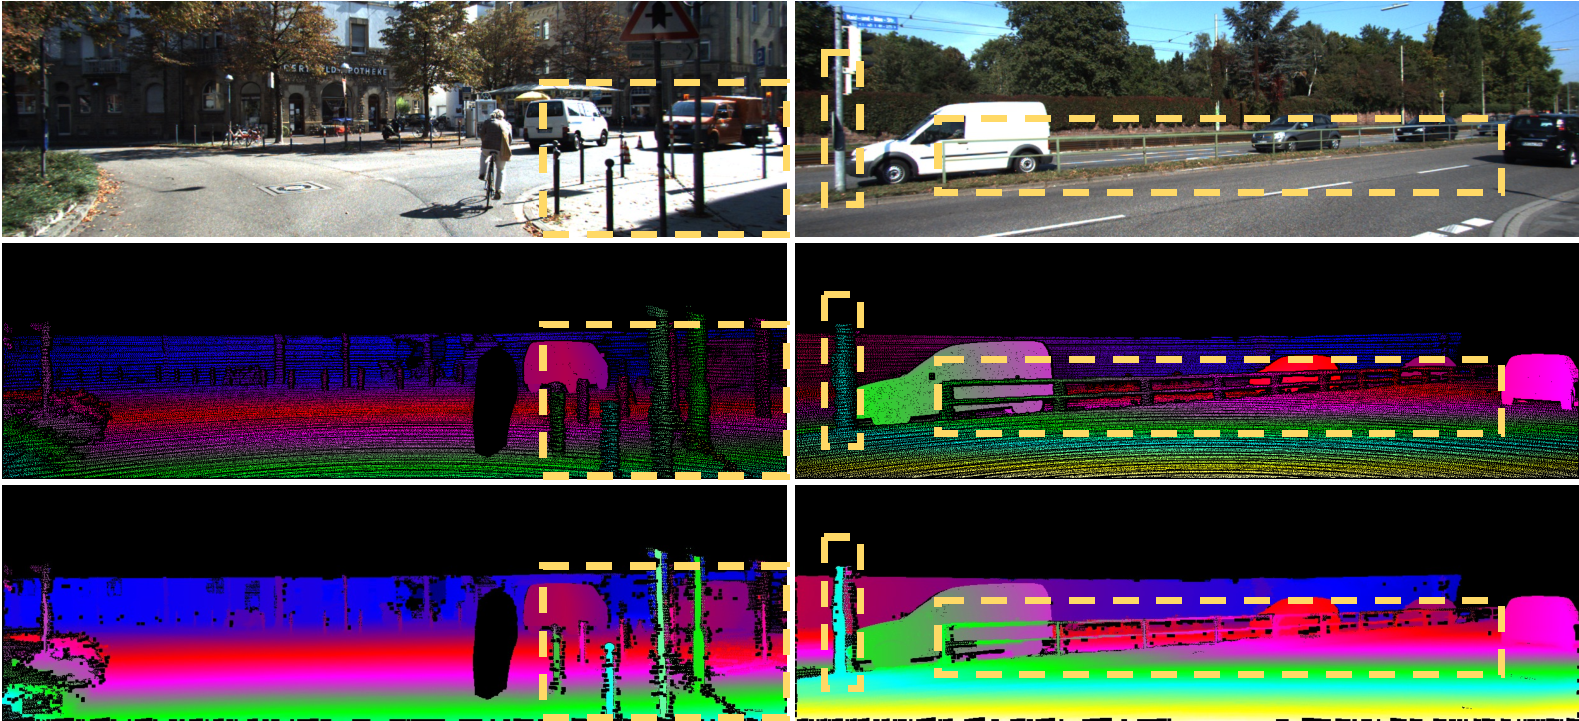
\includegraphics[width=0.99\linewidth]{fig/pseudo/pseudo.pdf}
	\vspace{-0.5em}
	\caption{
	\textbf{Depth Labels in KITTI.} First row: reference images, middle row: sparse ground-truth depth labels,
	last row: pseudo depth labels generated by our approach. Notably, ground truth depth labels suffer from thickening issues and our method restores the fine-grained structures from noisy ground truth labels. Black regions are ignored during training.
	}
	\label{fig:pseudo-labels}
	\vspace{-1.2em}
\end{figure}

\section{Experiments}

\subsection{Controlled Evaluation on KITTI-CARLA}

Evaluating pseudo-label quality on real-world datasets like KITTI is difficult because dense ground-truth disparities are not available for the benchmark test set, and the training labels are sparse and noisy.
Instead, we curate a synthetic datasets using KITTI-CARLA~\cite{deschaud2021kitticarla} to emulate KITTI's sparse and noisy depth annotations.
Following KITTI's data collection protocol, LiDAR points are integrated over a temporal window of 21 frames (spanning $[-10, +10]$ frames relative to the current frame) to generate sparse depth maps.
To simulate real-world measurement noise, perturbations are applied to LiDAR points and sensor poses during integration: Gaussian noise ($\sigma=1.5\,\mathrm{cm}$) is added to LiDAR points, while poses are perturbed with translational ($\sigma=2\,\mathrm{cm}$) and rotational ($\sigma=0.07^\circ$) random noise.
This procedure ensures depth maps exhibit sparsity and noise characteristics consistent with KITTI's ground truth.
The curated dataset is divided into 24,500 training and 10,500 test image pairs.
Sparse and noisy disparity maps are used for training and pseudo-label generation, while the precise KITTI-CARLA ground-truth disparities are reserved for evaluation.

Using the curated KITTI-CARLA dataset, we conduct a controlled experiment.
We compare two training strategies using the same NMRF architecture and hyperparameters.
The baseline model is trained directly with the sparse noisy labels.
The proposed model is trained with additional pseudo labels generated by structure-aware depth completion.
As shown in Table~\ref{tab:pseudo} (right), our additional pseudo labels bring a 32.3\% reduction in End-Point Error (EPE) and a 15.9\% improvement in the D1 metric (percentage of erroneous pixels with disparity error larger than 3 pixels and 5\% of the ground truth).
Qualitative results (Figure~\ref{fig:res_thin}) further demonstrate that pseudo-labels suppress the ``thickening'' artifacts, \ie, erroneous depth discontinuities induced by noisy supervision, yielding sharper object boundaries aligned with the reference image.
These results underscore the capability of pseudo labels to mitigate the label noise, enabling the model to achieve robust performance under imperfect real-world conditions.

Beyond disparity estimation, we evaluate the impact of pseudo label generation on surface normal quality, critical output for downstream 3D tasks (\eg, mesh reconstruction), obviating the need for an additional dedicated normal estimation network.
Surface normals are derived directly from disparity maps using camera intrinsic parameters, as described in~\cite{rossi2020joint}.
To isolate the effect of auxiliary loss (Equation~\ref{eq:loss-aux}), we train original NMRF and our adapted version on the SceneFlow dataset and evaluate normal errors on its test set.
Normal accuracy is quantified as the percentage of pixels with angular errors exceeding thresholds $t\in \{10^\circ,15^\circ,20^\circ,30^\circ\}$ (lower is better).
As reported in Table~\ref{tab:pseudo}, our auxiliary supervision reduces the error rate under the $20^\circ$ threshold by 35.6\%, confirming that our auxiliary supervision grounded on energy-based optimization enforces geometric consistency crucial for accurate normal derivation.
This highlights the broader utility of neural-energy fusion in learning geometrically coherent representation for robotic perception.
\begin{table}[t!]
	\centering
	\footnotesize
	\caption{Left: surface normal evaluation on the SceneFlow~\cite{mayer2016large}, where normal maps are derived from disparity estimates using the approach in~\cite{rossi2020joint}. Right: disparity evaluation on curated KITTI-CARLA dataset~\cite{deschaud2021kitticarla}. Bold values indicate the better performance for each metric.}
	\resizebox{0.99\linewidth}{!}{
		%\setlength\tabcolsep{2pt}
		\renewcommand\arraystretch{1.05}
		\begin{tabular}{l|cccc|cccc}
			\toprule
			\multirow[c]{2}{*}{Methods}
			& \multicolumn{4}{c|}{SceneFlow~\cite{mayer2016large}}
			& \multicolumn{4}{c}{Curated KITTI-CARLA~\cite{deschaud2021kitticarla}}\\
			%\cmidrule{2-9}
			\cline{2-9}
			& {\scriptsize $10^\circ$} & {\scriptsize $15^\circ$} & {\scriptsize $20^\circ$} & {\scriptsize $30^\circ$}
			& EPE & D1 & bad 1 & bad 3\\
			\midrule
			NMRF~\cite{guan2024neural} & 55.33 & 43.20 & 34.91 & 24.18 & 0.96 & 4.98 & 6.95 & 5.07\\
			Ours & \textbf{38.92} & \textbf{28.92} & \textbf{22.49} & \textbf{14.83} & \textbf{0.65} & \textbf{4.19} & \textbf{6.53} & \textbf{4.35}\\
			\bottomrule
		\end{tabular}
	}
	\label{tab:pseudo}
\end{table}

\begin{figure}[!t]
	\centering
	\tabcolsep=0.03cm
	\begin{tabular}{c c}
		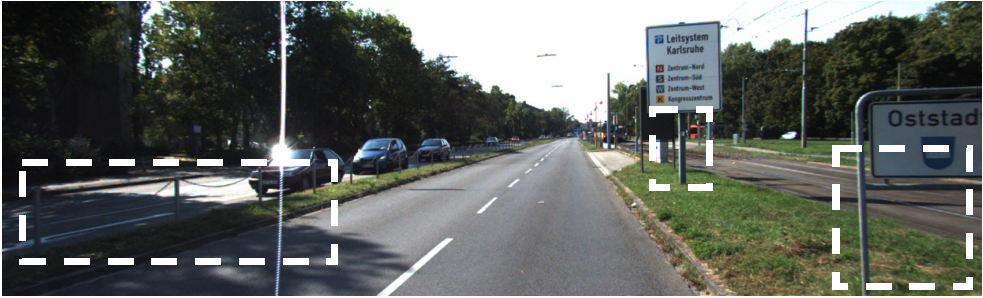
\includegraphics[width=0.49\linewidth]{fig/pseudo/thin_rgb.pdf}& 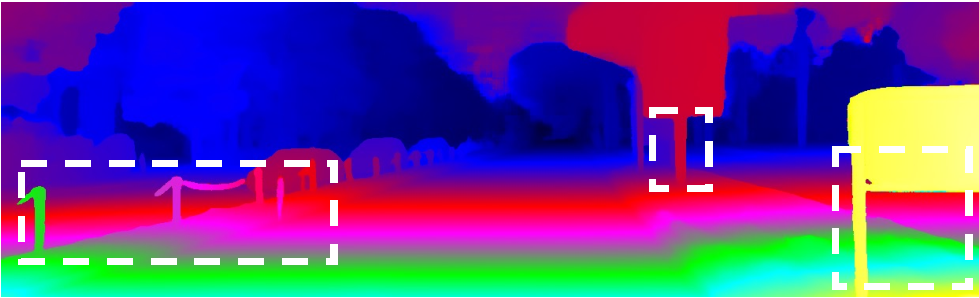
\includegraphics[width=0.49\linewidth]{fig/pseudo/thin_nmrf.pdf}\vspace{-1.0mm}\\ 
		(a) \textsf{\footnotesize Reference image} & (b) \textsf{\footnotesize NMRF~\cite{guan2024neural}}\\ 
		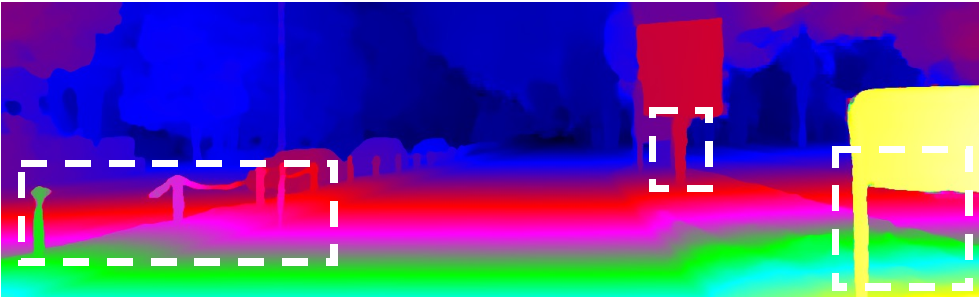
\includegraphics[width=0.49\linewidth]{fig/pseudo/thin_igev.pdf}& 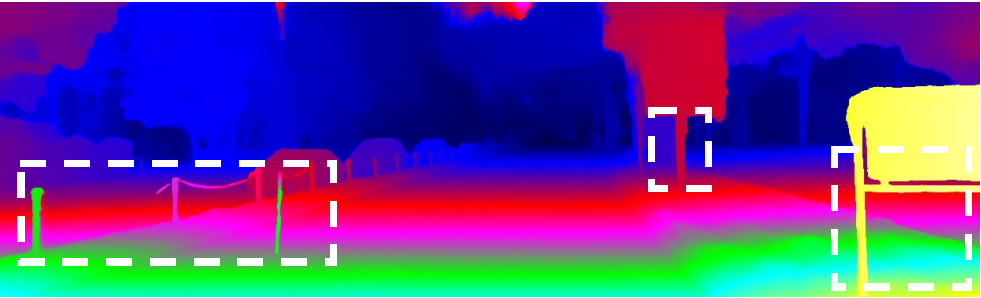
\includegraphics[width=0.49\linewidth]{fig/pseudo/thin_ours.pdf}\vspace{-1.0mm}\\
		(c) \textsf{\footnotesize IGEV~\cite{xu2023iterative}} & (d) \textsf{\footnotesize Ours}
	\end{tabular}
	%\vspace{-0.8em}
	\caption{\textbf{Qualitative results on KITTI benchmark.} Noisy ground truth depth labels lead to overly thickening object boundaries, even in state-of-the-art models~\cite{guan2024neural,xu2023iterative}. Our pseudo label supervision approach effectively mitigates this issue, preserving thin structures and holes.}
	\label{fig:res_thin}
	\vspace{-1.2em}
\end{figure}